\section{Results}
\subsection{Covariance estimation}
The covariance matrix is defined as
\begin{equation}\label{eq:true-covariance}
    \Sigma = \E{(x-\mu)(x-\mu)^\T},\quad \mu = \E{x}
\end{equation}
where $\E{\cdot}$ denotes expectation; the $p\times 1$ vector $x$ is a single observation of the firing rates of $p$ neurons in a time bin of some duration; and $\mu$ is the vector of expected firing rates.

Given a set of observations $\{x(t): t\in T$\} of population activity, where $x(t)$ is a $p\times 1$ vector of firing rates in time bin $t$, and an independent unbiased estimate $\bar x$ of the mean activity, the \emph{sample covariance matrix},
\begin{equation}\label{eq:sample}
   C_{\sf sample} = \frac 1 n \sum\limits_{t\in T} (x(t)-\bar x)(x(t)-\bar x)^\T,
\end{equation}
where $n$ is the number of time bins in $T$, yields an unbiased estimate of the covariance matrix so that $\E{C_{\sf sample}}=\Sigma$.

When the mean is estimated from the same sample, $C_{\sf sample}$ becomes biased toward zero.  However, in all the cases when the unbiasedness is required in our study, the mean will be estimated from a separate sample.

Given any covariance matrix estimate $C$, the corresponding correlation matrix $R$ is calculated by normalizing the rows and columns of $C$ by the square roots of its diagonal elements to produce unit entries on the diagonal:
\begin{equation}\label{eq:precision}
R = \left(I\circ C\right)^{-\frac 1 2} C \left(I\circ C\right)^{-\frac 1 2},
\end{equation}
where $\circ$ denotes the entrywise matrix product (Hadamard product) and $I$ is the $p\times p$ identity matrix.

The \emph{partial correlation} between a pair of variables is the Pearson correlation coefficient of the residuals of the linear least-squares predictor of their activity based on all the other variables, excluding the pair \citep{Anderson:2003, Whittaker:1990}. Partial correlations figure prominently in probabilistic \emph{graphical modeling} wherein the joint distribution is explained by sets of two-way interactions \citep{Whittaker:1990}. For the multivariate Gaussian distribution, zero partial correlations indicate conditional independence of the pair, implying a lack of direct interaction \citep{Dempster:1972, Whittaker:1990}. More generally, partial correlations can serve as a measure of conditional independence under the assumption that most dependencies in the system include strong linear effects \citep{Whittaker:1990,Baba:2004}. As neural recordings become increasingly dense, partial correlations may prove useful as indicators of conditional independence (lack of functional connectivity) between pairs of neurons.

Pairwise partial correlations are closely related to the elements of the \emph{precision matrix}, \emph{i.e.}\;the inverse of the covariance matrix \citep{Dempster:1972,Whittaker:1990}. Zero elements in the precision matrix signify zero partial correlation between the two variables. Given the covariance estimate $C$, the matrix of partial correlations $P$ is computed by normalizing the rows and columns of the \emph{precision matrix} $C^{-1}$ to produce negative unit entries on the diagonal:
\begin{equation}\label{eq:partial}
    P = -\left(I\circ C^{-1}\right)^{-\frac 1 2} C^{-1} \left(I\circ C^{-1}\right)^{-\frac 1 2}
\end{equation}

As the size of recorded neuronal populations increases, without substantial increases in recording durations, the \emph{condition number} of the sample covariance matrix also increases, making the partial correlation estimates \emph{ill-conditioned}: small errors in covariance estimates translate into much greater errors in partial correlations after the inversion. With massively multineuronal recordings, partial correlations cannot be estimated without \emph{regularization} \citep{Ledoit:2004,Schafer:2005}.

We considered four regularized estimators based on distinct families of target estimates: $C_{\sf diag}$, $C_{\sf factor}$, $C_{\sf sparse}$, and $C_{\sf sparse+latent}$. In probabilistic models with exclusively linear dependencies, the target estimates of these estimators correspond to distinct families of graphical models (Fig.~\ref{fig:1} Row 1).

\begin{figure}
\begin{leftfullpage}
\caption[Regularized correlation matrix estimators]{{\bf Regularized correlations matrix estimators.}
{\bf Regularized estimators whose structure matches the true structure in the data are more efficient.}
     {\bf Row 1.} Graphical models of the target estimates of the four respective regularized covariance matrix estimators.  Recorded neurons are represented by the green spheres and latent units by the lightly shaded spheres.  Edges represent conditional dependencies, \emph{i.e.}\;`interactions'.
     {\bf Row 1, A}.  For estimator $C_{\sf diag}$, the target estimate is a diagonal matrix, which describes systems that lack linear dependencies.
     {\bf  Row 1, B.} For estimator $C_{\sf factor}$, the target estimate is a factor model (low-rank matrix plus a diagonal matrix), representing systems in which correlations arise due to common input from latent units.
     {\bf  Row 1, C}. For estimator $C_{\sf sparse}$, the covariance matrix is approximated as the inverse of a sparse matrix. This approximation describes systems in which correlations arise from a sparse set of  linear associations between the observed units.
     {\bf  Row 1, D}.  For estimator $C_{\sf sparse+latent}$, the covariance matrix is approximated as the inverse of the sum of a sparse matrix and a low-rank matrix. This approximation describes a model wherein correlations arise due to sparse associations between the recorded cells \emph{and} due to several latent units.
     \\
     {\bf Row 2:} Examples of $50\times 50$ correlation matrices corresponding to each structure: {\bf A.} the diagonal correlation matrix, {\bf B.} a factor model with four latent units, {\bf C.}  a correlation matrix with 67\%  off-diagonal zeros in its inverse, and {\bf  D.} a correlation matrix whose inverse is the sum of a rank-3 matrix (\emph{i.e.}\;three latent units) and a sparse matrix with 76\% off-diagonal zeros.
     \\
{\bf Row 3:} Sample correlation matrices calculated from samples of size $n=500$ drawn from simulated random processes with respective correlation matrices shown in Row 2.  The structure of the sample correlation matrix is difficult to discern by eye.
     \\
{\bf Row 4:} Estimates computed from the same data as in Row 3 using structured estimators of the correct type, optimized by cross-validation.  The regularized estimates are closer to the truth than the sample correlation matrices.
     \\
{\bf Row 5:} True loss (Eq.~\ref{eq:loss}) for the five estimators as a function of sample size. The error bars indicate the standard deviation of the mean.  Estimators with structure that matches the true model converged to zero faster than the other estimators.
     \\
{\bf Row 6:} Validation loss (Eq.~\ref{eq:vloss}) for the five estimators relative to the matching estimators for each type of ground truth. Error bars indicate the standard deviation of the mean.  Differences in validation loss approximate differences in true loss.
}\label{fig:1}
\end{leftfullpage}
\end{figure}

\begin{figure}
\begin{fullpage}
        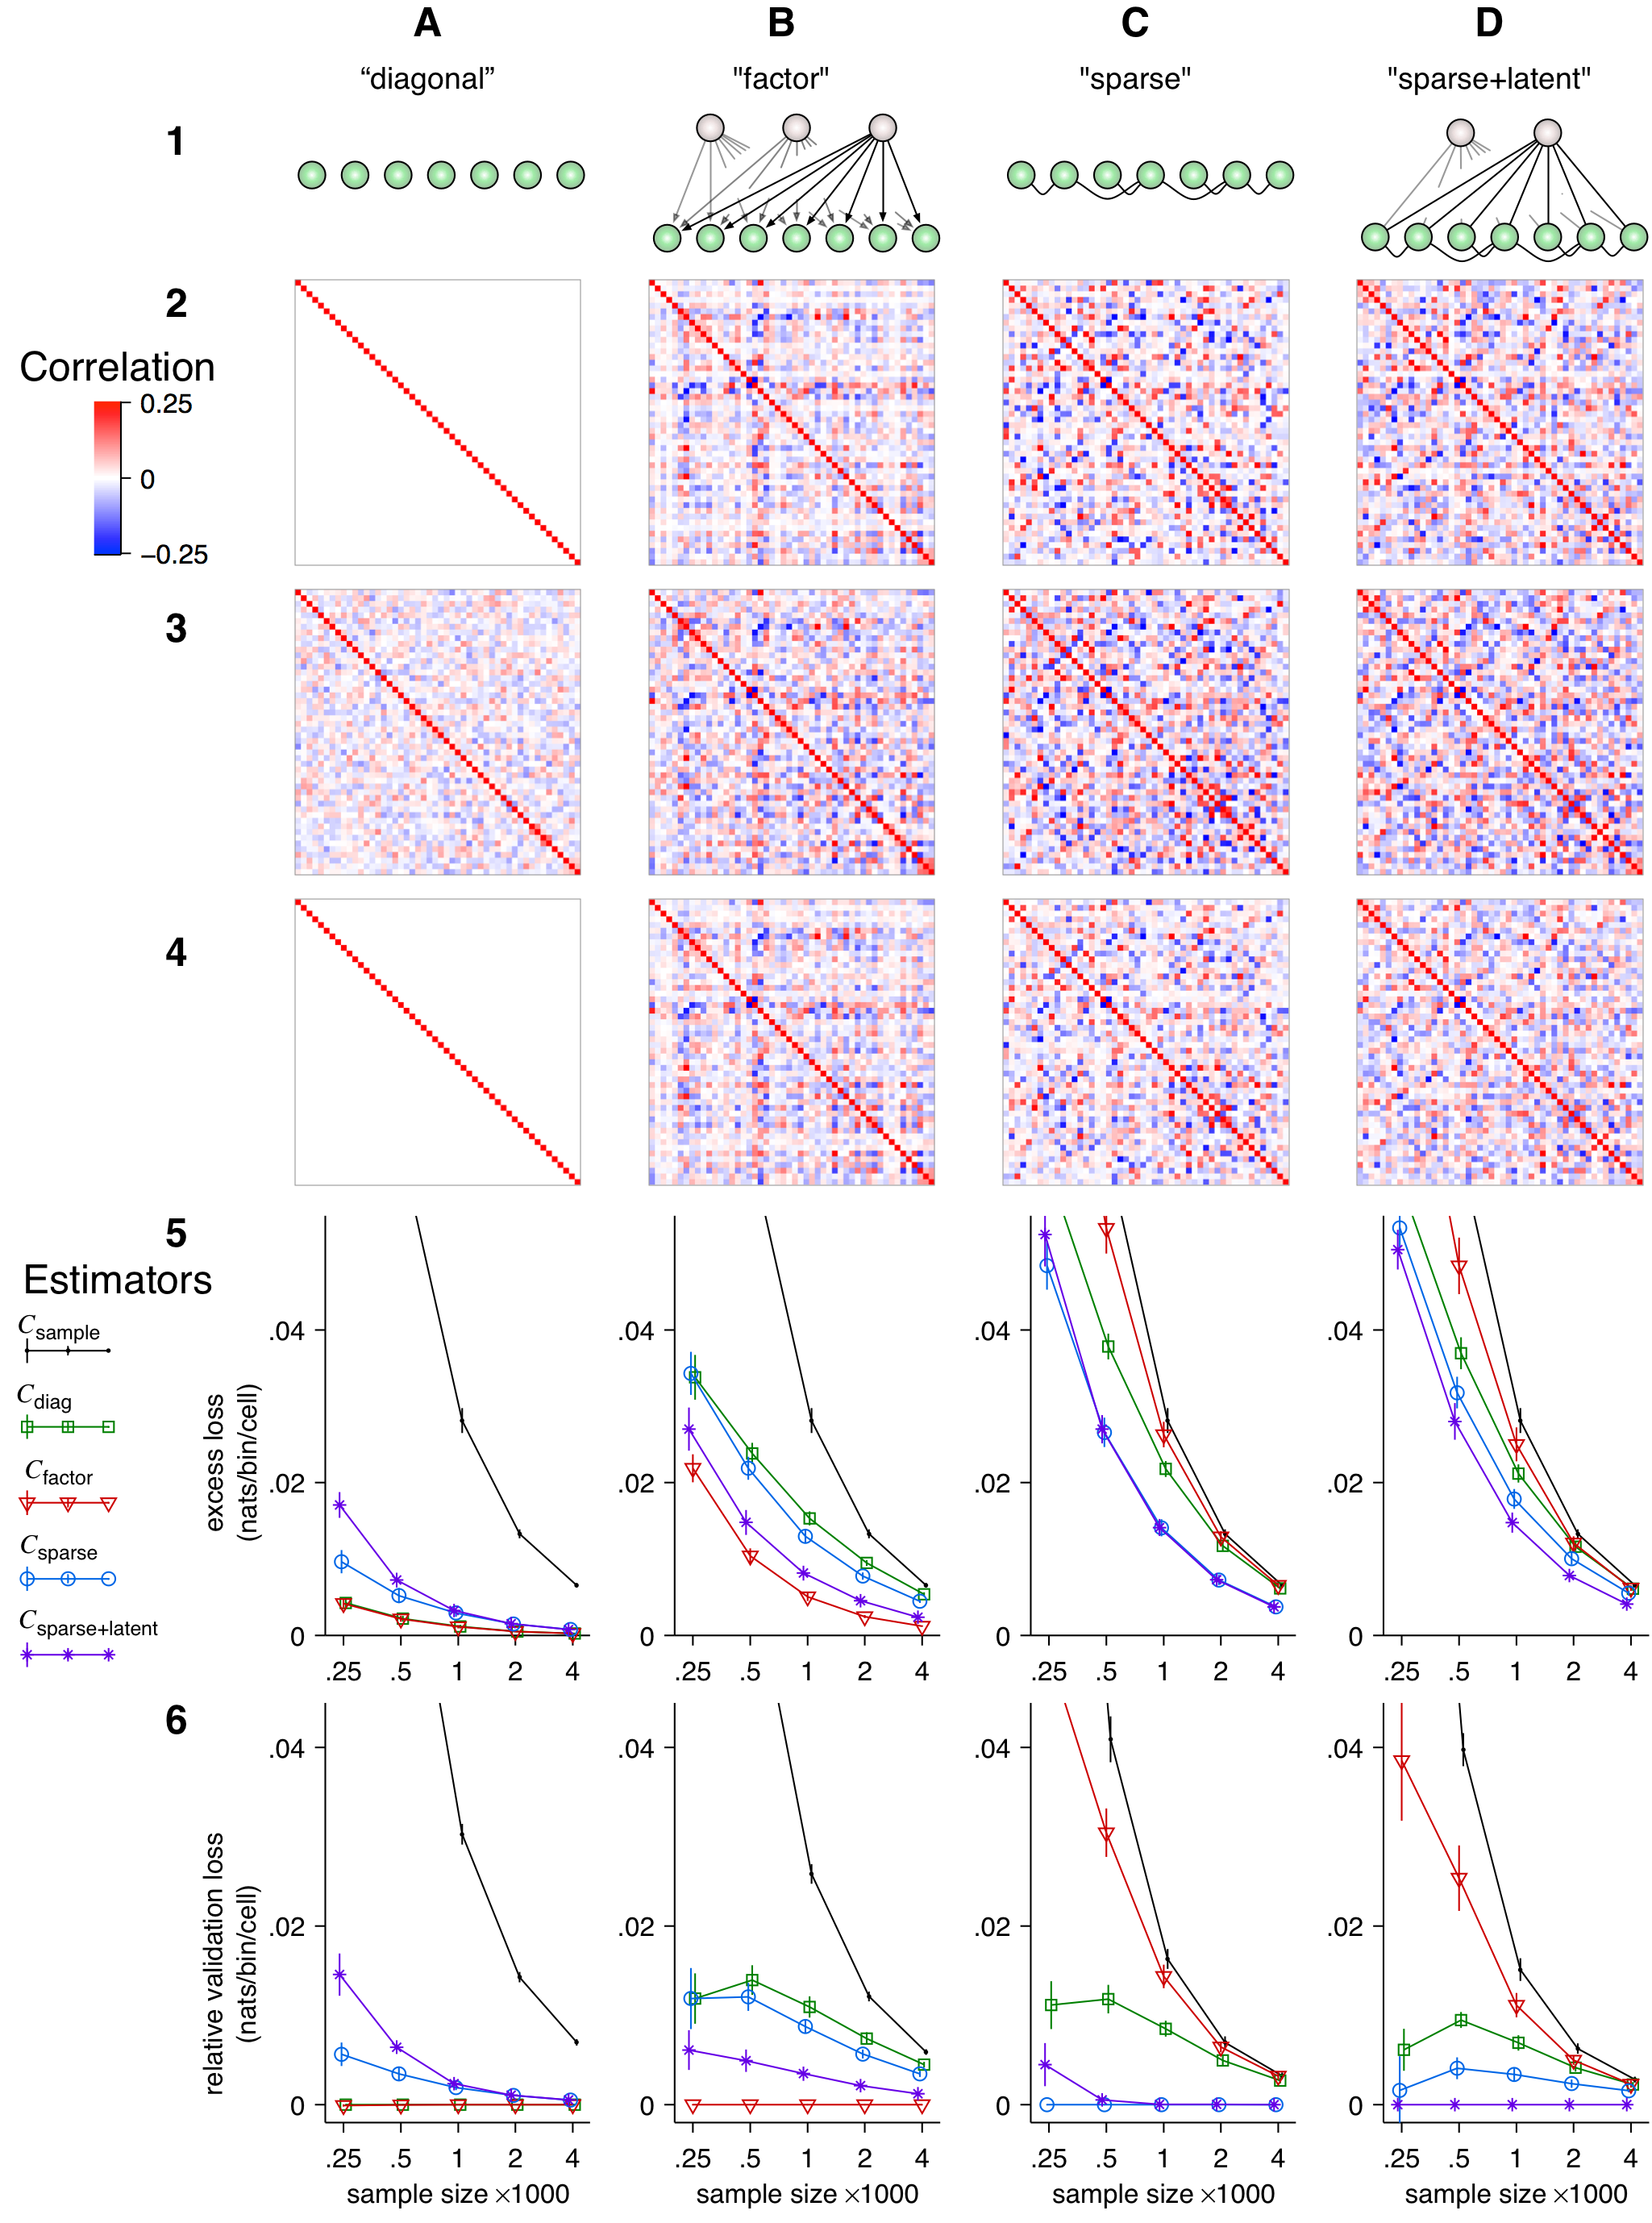
\includegraphics[width=\textwidth]{./figures/Figure1.png}
\end{fullpage}
\end{figure}
  %%%%%%%%%%%% Figure 1

The target estimate of estimator $C_{\sf diag}$ is the diagonal matrix $D$ containing estimates of neurons' variances. Regularization is achieved by linear \emph{shrinkage} of the unbiased estimate $C_{\sf sample}$ toward $D$ controlled by the scalar \emph{shrinkage intensity} parameter $\lambda \in [0, 1]$:
\begin{equation}\label{eq:c-diag}
    C_{\sf diag} = (1-\lambda) C_{\sf sample} + \lambda D
\end{equation}
The structure imposed by $C_{\sf diag}$ favors (performs better  on) populations   with no linear associations between the neurons (Fig.~\ref{fig:1} Row 1, A).  If sample correlations are largely spurious, $C_{\sf diag}$ is expected to be more efficient than other estimators.

Estimator $C_{\sf factor}$ approximates the covariance matrix by the factor model $L + D$, where $L$ is the $p\times p$ positive semidefinite matrix of a low rank and $D$ is a diagonal matrix of independent variances. This approximation is the basis for \emph{factor analysis} \citep{Anderson:2003}. The estimator,
\begin{equation}\label{eq:c-factor}
    C_{\sf factor} = L + (1-\lambda)D + \lambda \bar D,
\end{equation}
has two hyperparameters: the rank of $L$ (\emph{i.e.}\;the number of latent factors) and the shrinkage intensity $\lambda$ to shrink the independent variances toward their mean value $\bar D$. The structure imposed by $C_{\sf factor}$ favors conditions in which the population activity is linearly driven by a number of latent factors that affect many cells while direct interactions between the recorded cells are insignificant (Fig.~\ref{fig:1} Row 1, B).

Estimator $C_{\sf sparse}$ is produced by approximating the sample covariance matrix by the inverse of a sparse matrix $S$:
\begin{equation}\label{eq:c-sparse}
    C_{\sf sparse} = S^{-1}.
\end{equation}
Here $S$ is a sparse matrix, \emph{i.e.}\;one in which a large fraction of off-diagonal elements are set to zero.  The estimator has one hyperparameter that determines the sparsity (fraction of off-diagonal zeros) in $S$. The problem of finding the optimal set of non-zero elements of the precision matrix is known as \emph{covariance selection} \citep{Dempster:1972}. The structure imposed by $C_{\sf sparse}$ favors conditions in which neural correlations arise from direct linear effects (`interactions') between some pairs of neurons (Fig.~\ref{fig:1}} Row 1, C).

Estimator $C_{\sf sparse+latent}$ is obtained by approximating the sample covariance matrix by a matrix whose inverse is the sum of a sparse component and a low-rank component:
\begin{equation}\label{eq:c-sl}
    C_{\sf sparse+latent} = (S - L)^{-1},
\end{equation}
where, as above, $S$ is a sparse matrix and $L$ is a low-rank matrix. The estimator has two hyperparameters: one to regulate the sparsity of $S$ and the other to regulate the rank of $L$. See Methods for a more detailed explanation. The structure imposed by $C_{\sf sparse+latent}$ favors conditions in which the activity of neurons is determined by linear effects between some observed pairs of neurons and linear effects from several latent units (Fig.~\ref{fig:1} Row 1, D) \citep{Chandrasekaran:2010,Ma:2013}.

We refer to the sparse partial correlations in estimators $C_{\sf sparse}$ and $C_{\sf sparse+latent}$ as `interactions'.
